% !TEX root = ../tesi.tex
%
\chapter{The ALICE experiment}
\label{sec:3}

\cleanchapterquote{To see a World in a Grain of Sand \\
                   And a Heaven in a Wild Flower \\ 
                   Hold Infinity in the palm of your hand \\
                   And Eternity in an hour}{William Blake}{(Auguries of Innocence)}

The Large Hadron Collider (LHC) is the biggest and more powerful particle collider in the world.
It consists of a 27 km ring of superconducting magnets and accelerating structures able to
provides proton-proton and Lead-Lead collisions at the highest energies ever reached in laboratory
to which the formation of the Quark Gluon Plasma is expected.
While most of the LHC uptime is dedicated to the proton–proton physics that led to the discovery of 
the Higgs Boson \cite{atlashiggs,cmshiggs} and of two charmed pentaquark states \cite{lhcbpenta}, 
a significant part of the physics programme at the LHC is dedicated to heavy-ion physics and the 
characterisation of the Quark Gluon Plasma.

\section{The Large Hadron Collider} \label{sec:3.1}

The Large Hadron Collider is the last element of the accelerator complex at CERN (Figure \ref{fig:lhc})
, a succesion of machines that accelerate particles to increasingly higher energies. Each element in
this chain boosts the energy of a beam of particles, before injecting it into the next machine. 
Protons and heavy ions are brought to their collision energies through different acceleration chains.

\begin{figure}
    \centering
    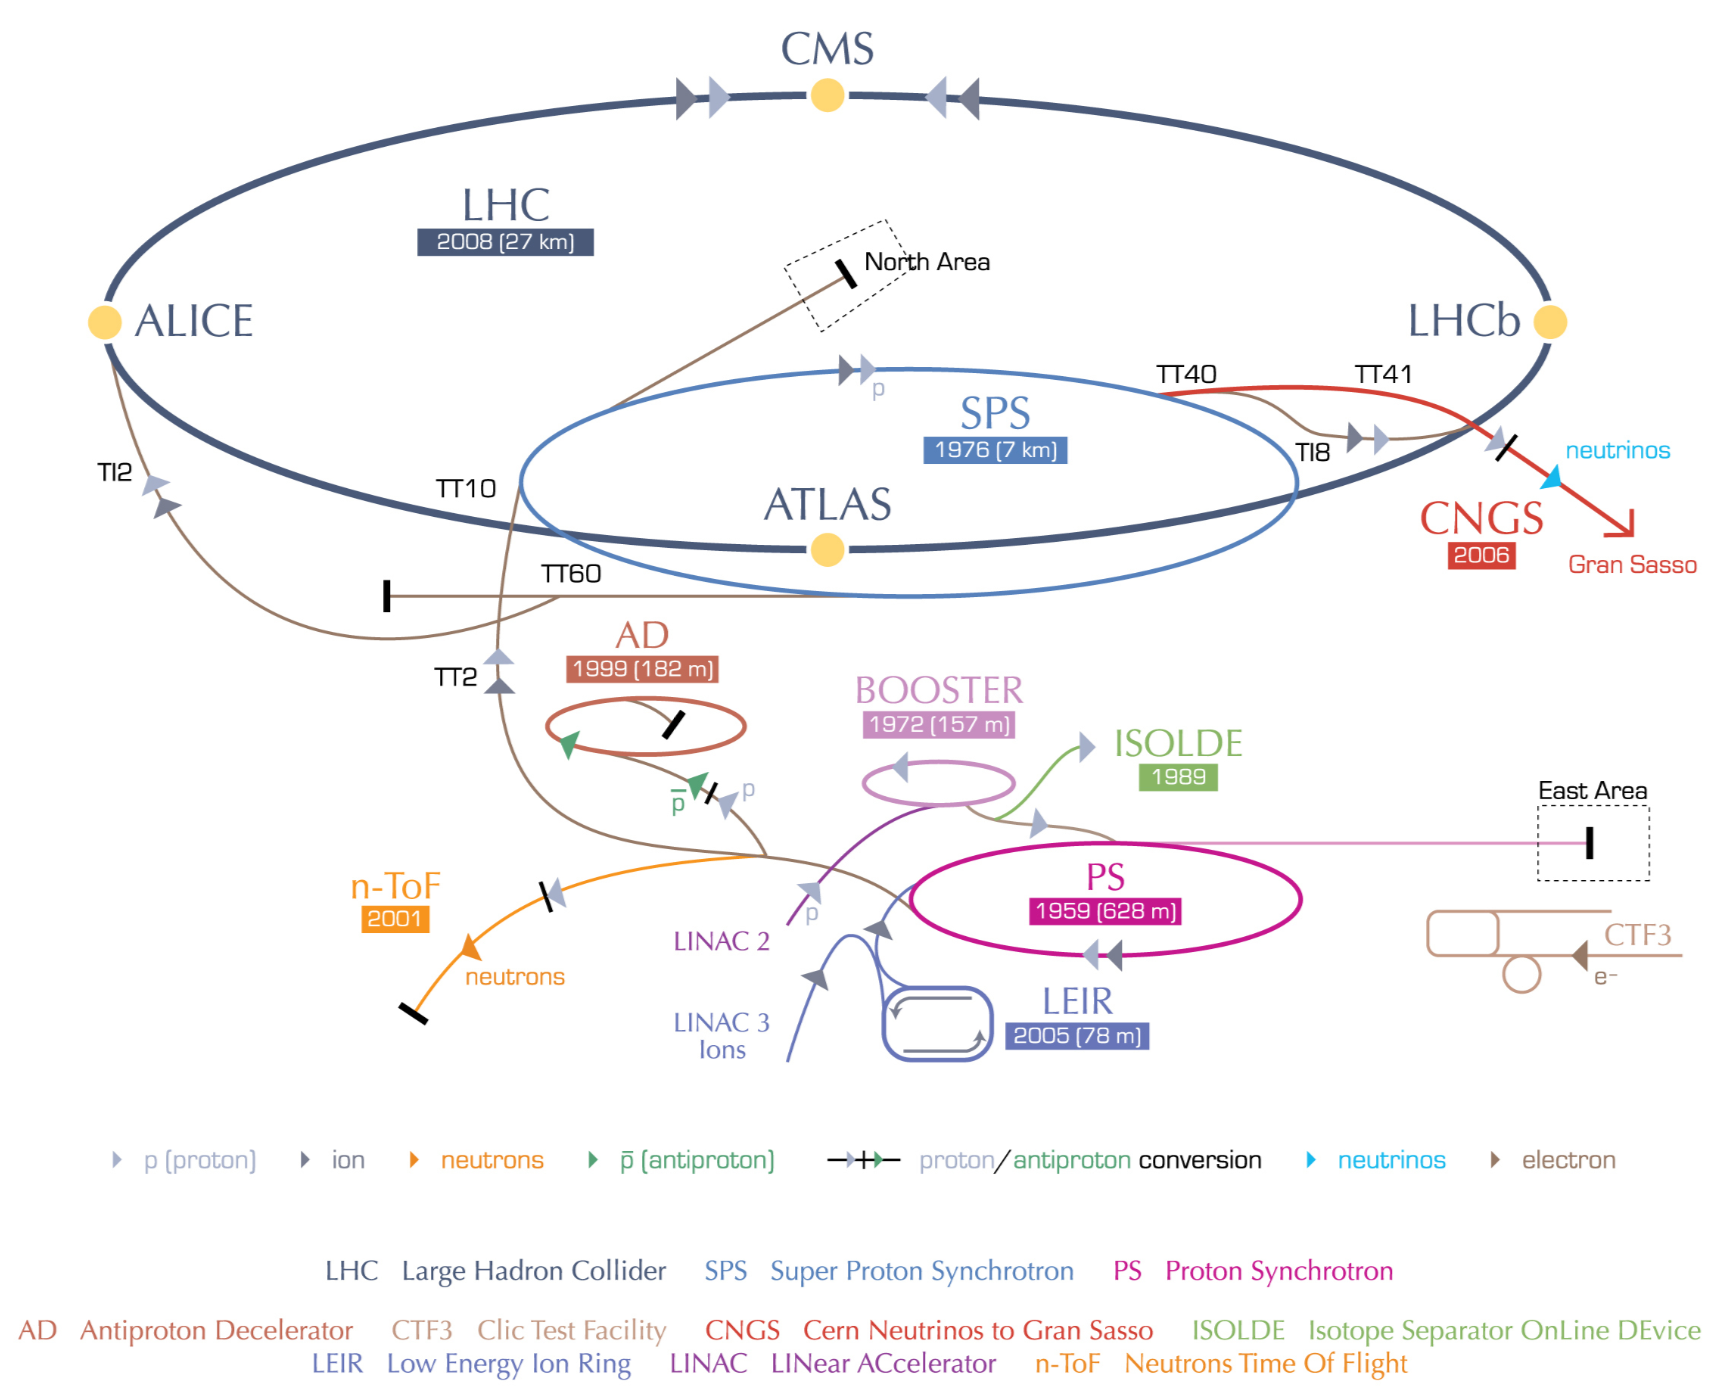
\includegraphics[width=0.8\textwidth]{gfx/lhc}
	\caption{Schematic view of the CERN accelerator complex and the LHC experiments \cite{lhc}.}
	\label{fig:lhc}
\end{figure}

The protons injected in the LHC ring starts their journey in the LINAC2, where ionized hydrogen
atoms are accelereted up to 50 MeV. Then the beam is injected in the Proton Synchrotron Booster 
(PSB), which accelerates protons up to 1.4 GeV and provides the beam bunches to the Proton 
Synchrotron (PS). The Proton Synchrotron provides 25 GeV protons to the Super Proton Synchrotron
(SPS), where they are accelerated up to 450 GeV before the injection in the LHC.

Lead ions are produced from a highly isotopically pure $^{208}$Pb sample heated to a temperature
of about $800\,^{\circ}\mathrm{C}$.
The lead vapour is ionized by an electron current. Many different charge states are produced
with a maximum around Pb$^{29+}$.
These ions are selected and accelerated to 4.2 MeV/u (energy per nucleon) before passing through
a carbon foil, which strips most of them to Pb$^{54+}$. The Pb$^{54+}$ beam is accumulated, then
accelerated to 72 MeV/u in the Low Energy Ion Ring (LEIR), which transfers them to the PS.
The PS accelerates the beam to 5.9 GeV/u and sends it to the SPS after first passing it through a
second foil where it is fully stripped to Pb$^{82+}$. 
The SPS accelerates it to 177 GeV/u then sends it to the LHC, which accelerates it to 2.56 TeV/u.

The LHC ring is composed by 1232 dipole magnets and 392 quadrupole magnets, which respectively 
guide and focus the counter–rotating beams in separate vacuum–filled pipes.
When the beams are stable they are brought into collision in four interaction points corresponding
to the major LHC experiments.
The top centre–of–mass energy reached at the LHC in the collisions are 13 TeV and 5.02 TeV per 
nucleon pair for pp and Pb--Pb collisions respectively.

Besides the centre–of–mass energy another crucial parameter for a collider is the luminosity delivered 
to the experiment.
Indeed the number of events per second generated in the LHC collisions can be evaluated with the
following formula:
\begin{equation}
    R_{event} = L\;\sigma_{event}
\end{equation}
where $L$ is the machine instantaneous luminosity and $\sigma_{event}$ is the cross section for
the event under study. The instantaneous luminosity depends only on the beam parameters and can be 
written as:
\begin{equation}
    L = \frac{N_{b}N^{2} f_{rev} \gamma}{4\,\pi \epsilon_{n} \beta^{*}} F,
\end{equation}
where $N_{b}$ is the number of bunches in the collider ring, $N$ is the number of charges in each
bunch, $f_{rev}$ is the revolution frequency of the beam, $\gamma$ is the relativistic factor,
$\epsilon_{n}$ is the normalized emittance\footnote{$\epsilon_{n} = \beta \gamma \epsilon$ 
where $\beta$ and $\gamma$ are the usual relativistic factors and the emittance $\epsilon$ is the
spread of beam particles in the position-momentum phase space.} and $\beta^{*}$ is the value 
of the amplitude function\footnote{The amplitude function $\beta(s)$ describes the beam 
amplitude modulation due to the changing focusing strength.} at the interaction point (IP)
where the luminosity is estimated.

\begin{figure}
    \centering
    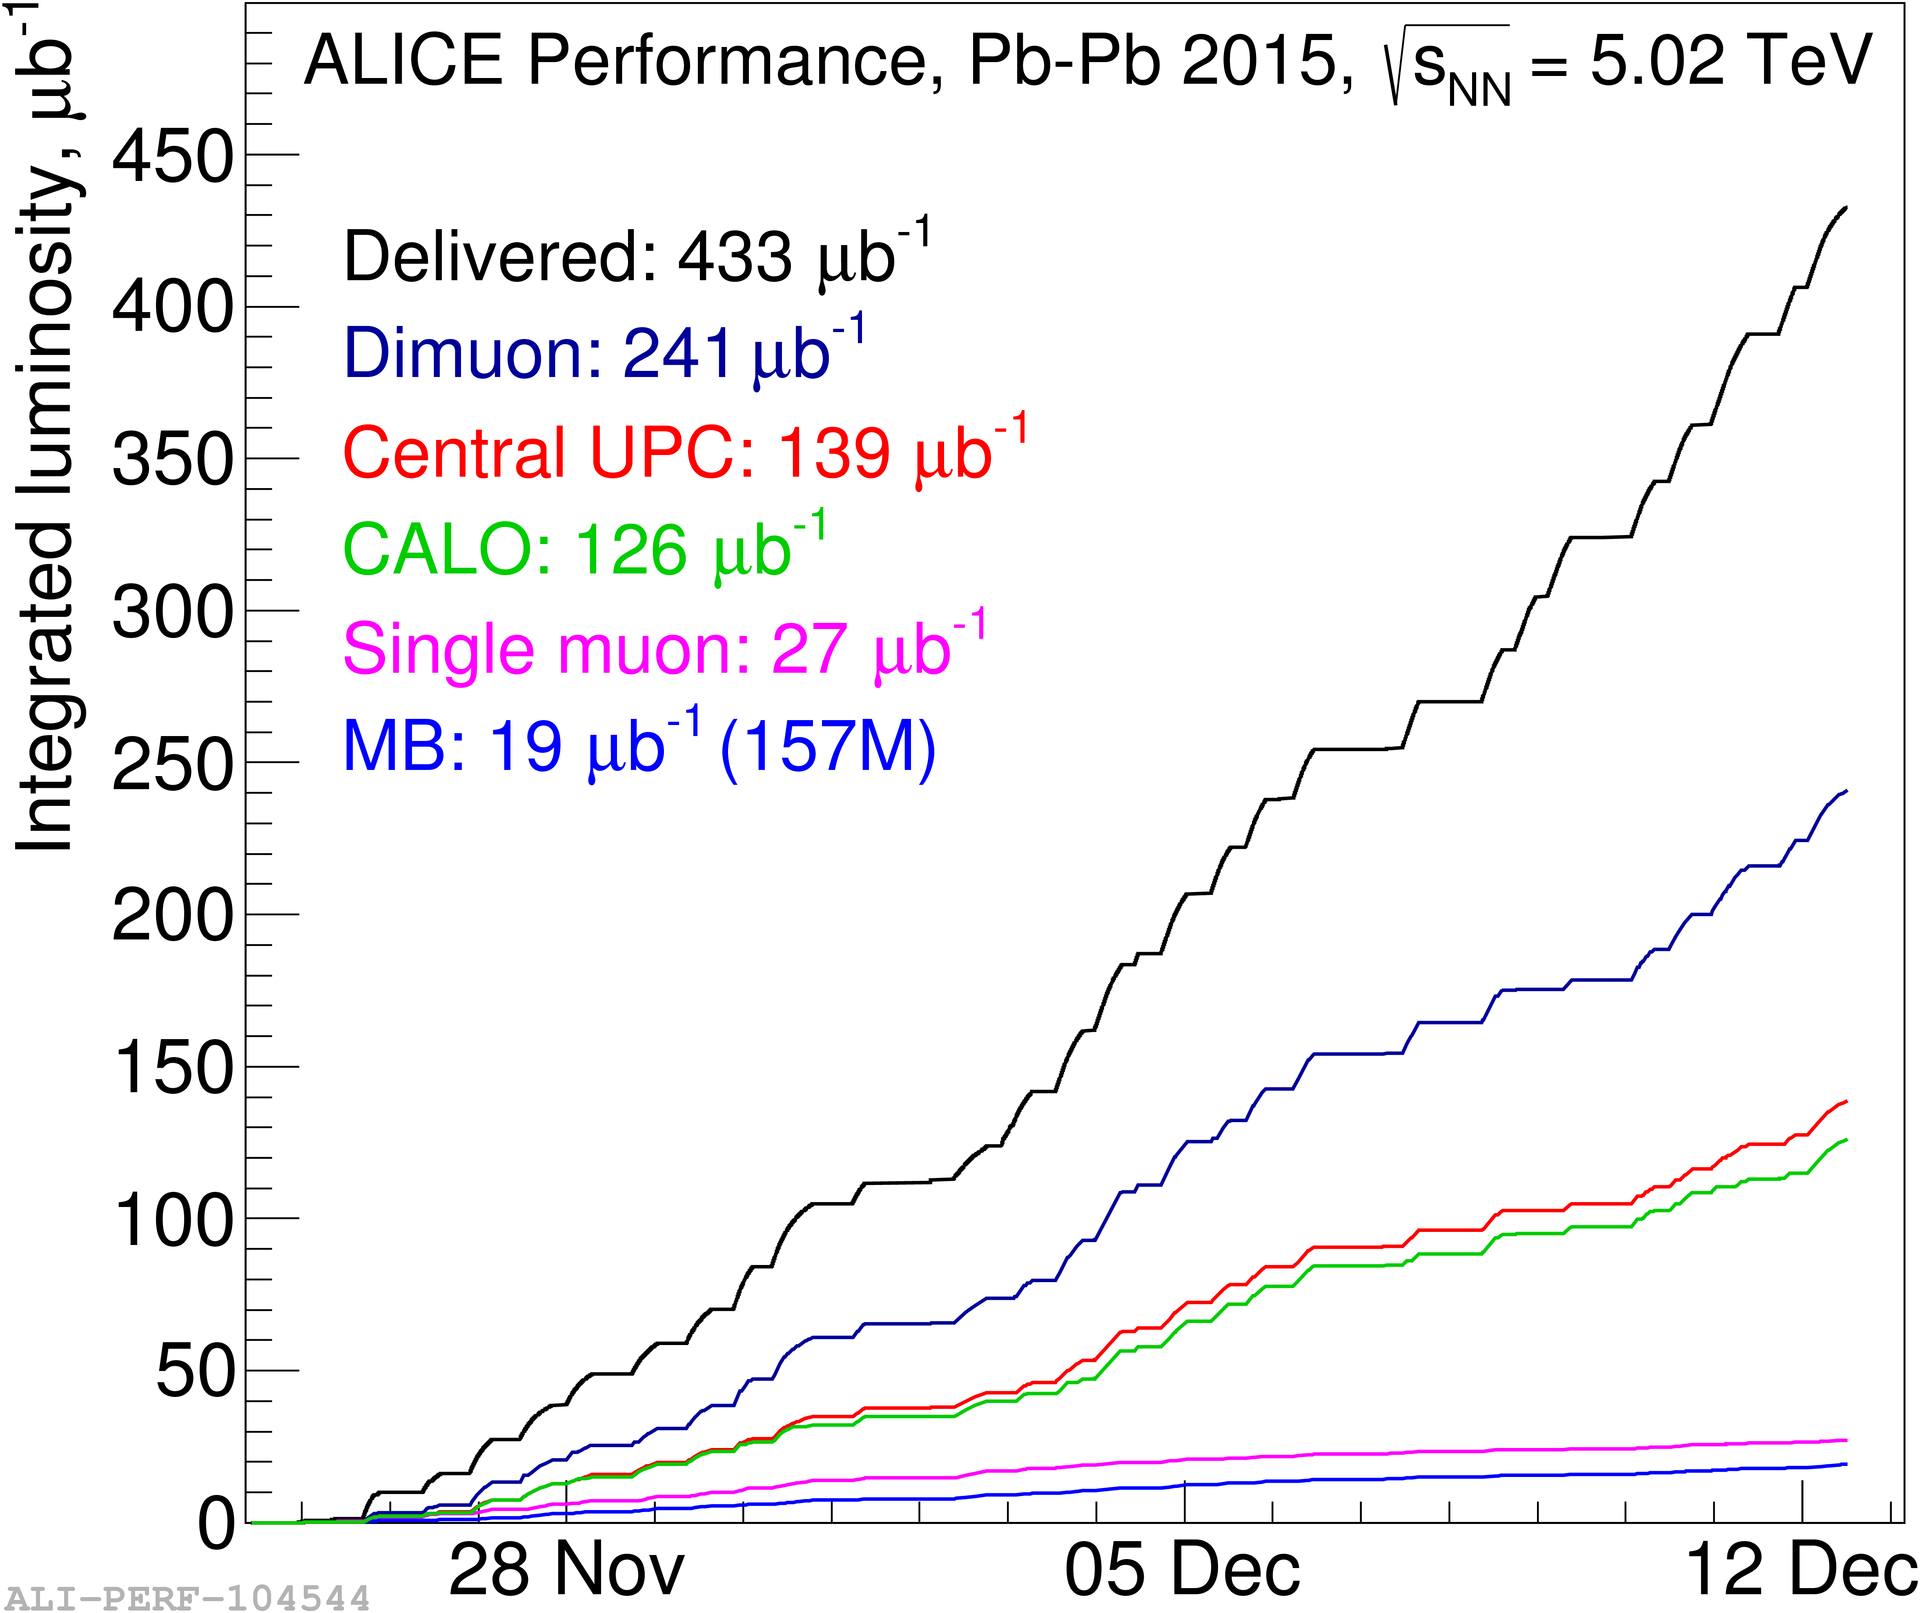
\includegraphics[width=0.6\textwidth]{gfx/alicelumi}
	\caption{ALICE delivered and integrated luminosity during the first Pb–Pb period in Run 2.}
	\label{fig:alicelumi}
\end{figure}

In order to maximise the luminosity of the LHC, the option of a p$\bar{\mathrm{p}}$ collider
was excluded due to the problem of the anti–protons production that is very complicated.
The LHC can store up to 2808 bunches, with $\sim 10^{11}$ protons per bunch, with 25 ns spacing
\cite{lhcperf}.
The ALICE apparatus requires a peak luminosity of $L = 10^{27}$ cm$^{-2}$s$^{-1}$ in Pb--Pb collisions.
Figure \ref{fig:alicelumi} shows the delivered luminosity by the LHC (black line) and the integrated
luminosities collected by ALICE, for different trigger configurations (colored lines), during the
first Pb–Pb period in Run 2 at the end of 2015.

A creucial information for the collider experiments is the the position where the collision
between the two beams takes place: the \textit{primary vertex}. 
The nominal position of the primary vertex is the origin of the coordinate reference frame of the 
experiment. Nevertheless, due to the finite size of the bunches the position of the primary
vertex fluctuates around the nominal position.
Being $\sigma^{bunch}_{x,y,z}$ the \textit{rms} of the bunch in the transverse and longitudinal
direction, it can be shown that, assuming a gaussian profile of the bunches in the three directions,
the \textit{rms} of the vertex variation is:
\begin{equation}
    \sigma^{vertex}_{x,y,z} = \frac{\sigma^{bunch}_{x,y,z}}{\sqrt{2}},
\end{equation}
where the \textit{rms} size depends on the beam emittance and the amplitude function $\beta^{*}$:
\begin{equation}
    \sigma^{bunch}_{x,y,z} = \sqrt{\frac{\epsilon_{x,y,z}\,\beta^{*}}{\sqrt{\pi}}}.
\end{equation}
At the IP2, where the ALICE experiment is located, typical values for the vertex dispersion are 
$\sigma^{vertex}_{x,y}\,\sim 50\;\mu\mathrm{m}$ and $\sigma^{vertex}_{z}\,\sim 5\;\mathrm{cm}$.

%
%
\section{ALICE design} \label{sec:3.2}

The main goal of the ALICE esperiment is the study of the QCD matter created in high energy heavy
ion collisions, hence has been specifically designed and optimised \cite{alicedesign1,alicedesign2}
for this purpose.
An heavy ion experiment must have an efficient tracking system with a large acceptance and a good
particle identification (PID) capabilities in a wide momentum range, expecially at low momentum.
Furthermore, it must work in an environment characterised by a large charged particle multiplicity.
At the time of ALICE design, the charged particles multiplicity per rapidity unit in central Pb–Pb 
collisions was predictied to range between 2000 and 8000 \cite{alicemulti}, and for this reason
detectors with high granularity and low material budget have been developed 
\cite{alicedesign1,alicedesign2}.

The current layout of the ALICE experiment is shown in Figure \ref{fig:alice3D} while Table 
\ref{tab:alice} lists the position and the purpose of the ALICE sub-detectors.
\begin{figure}
    \centering
    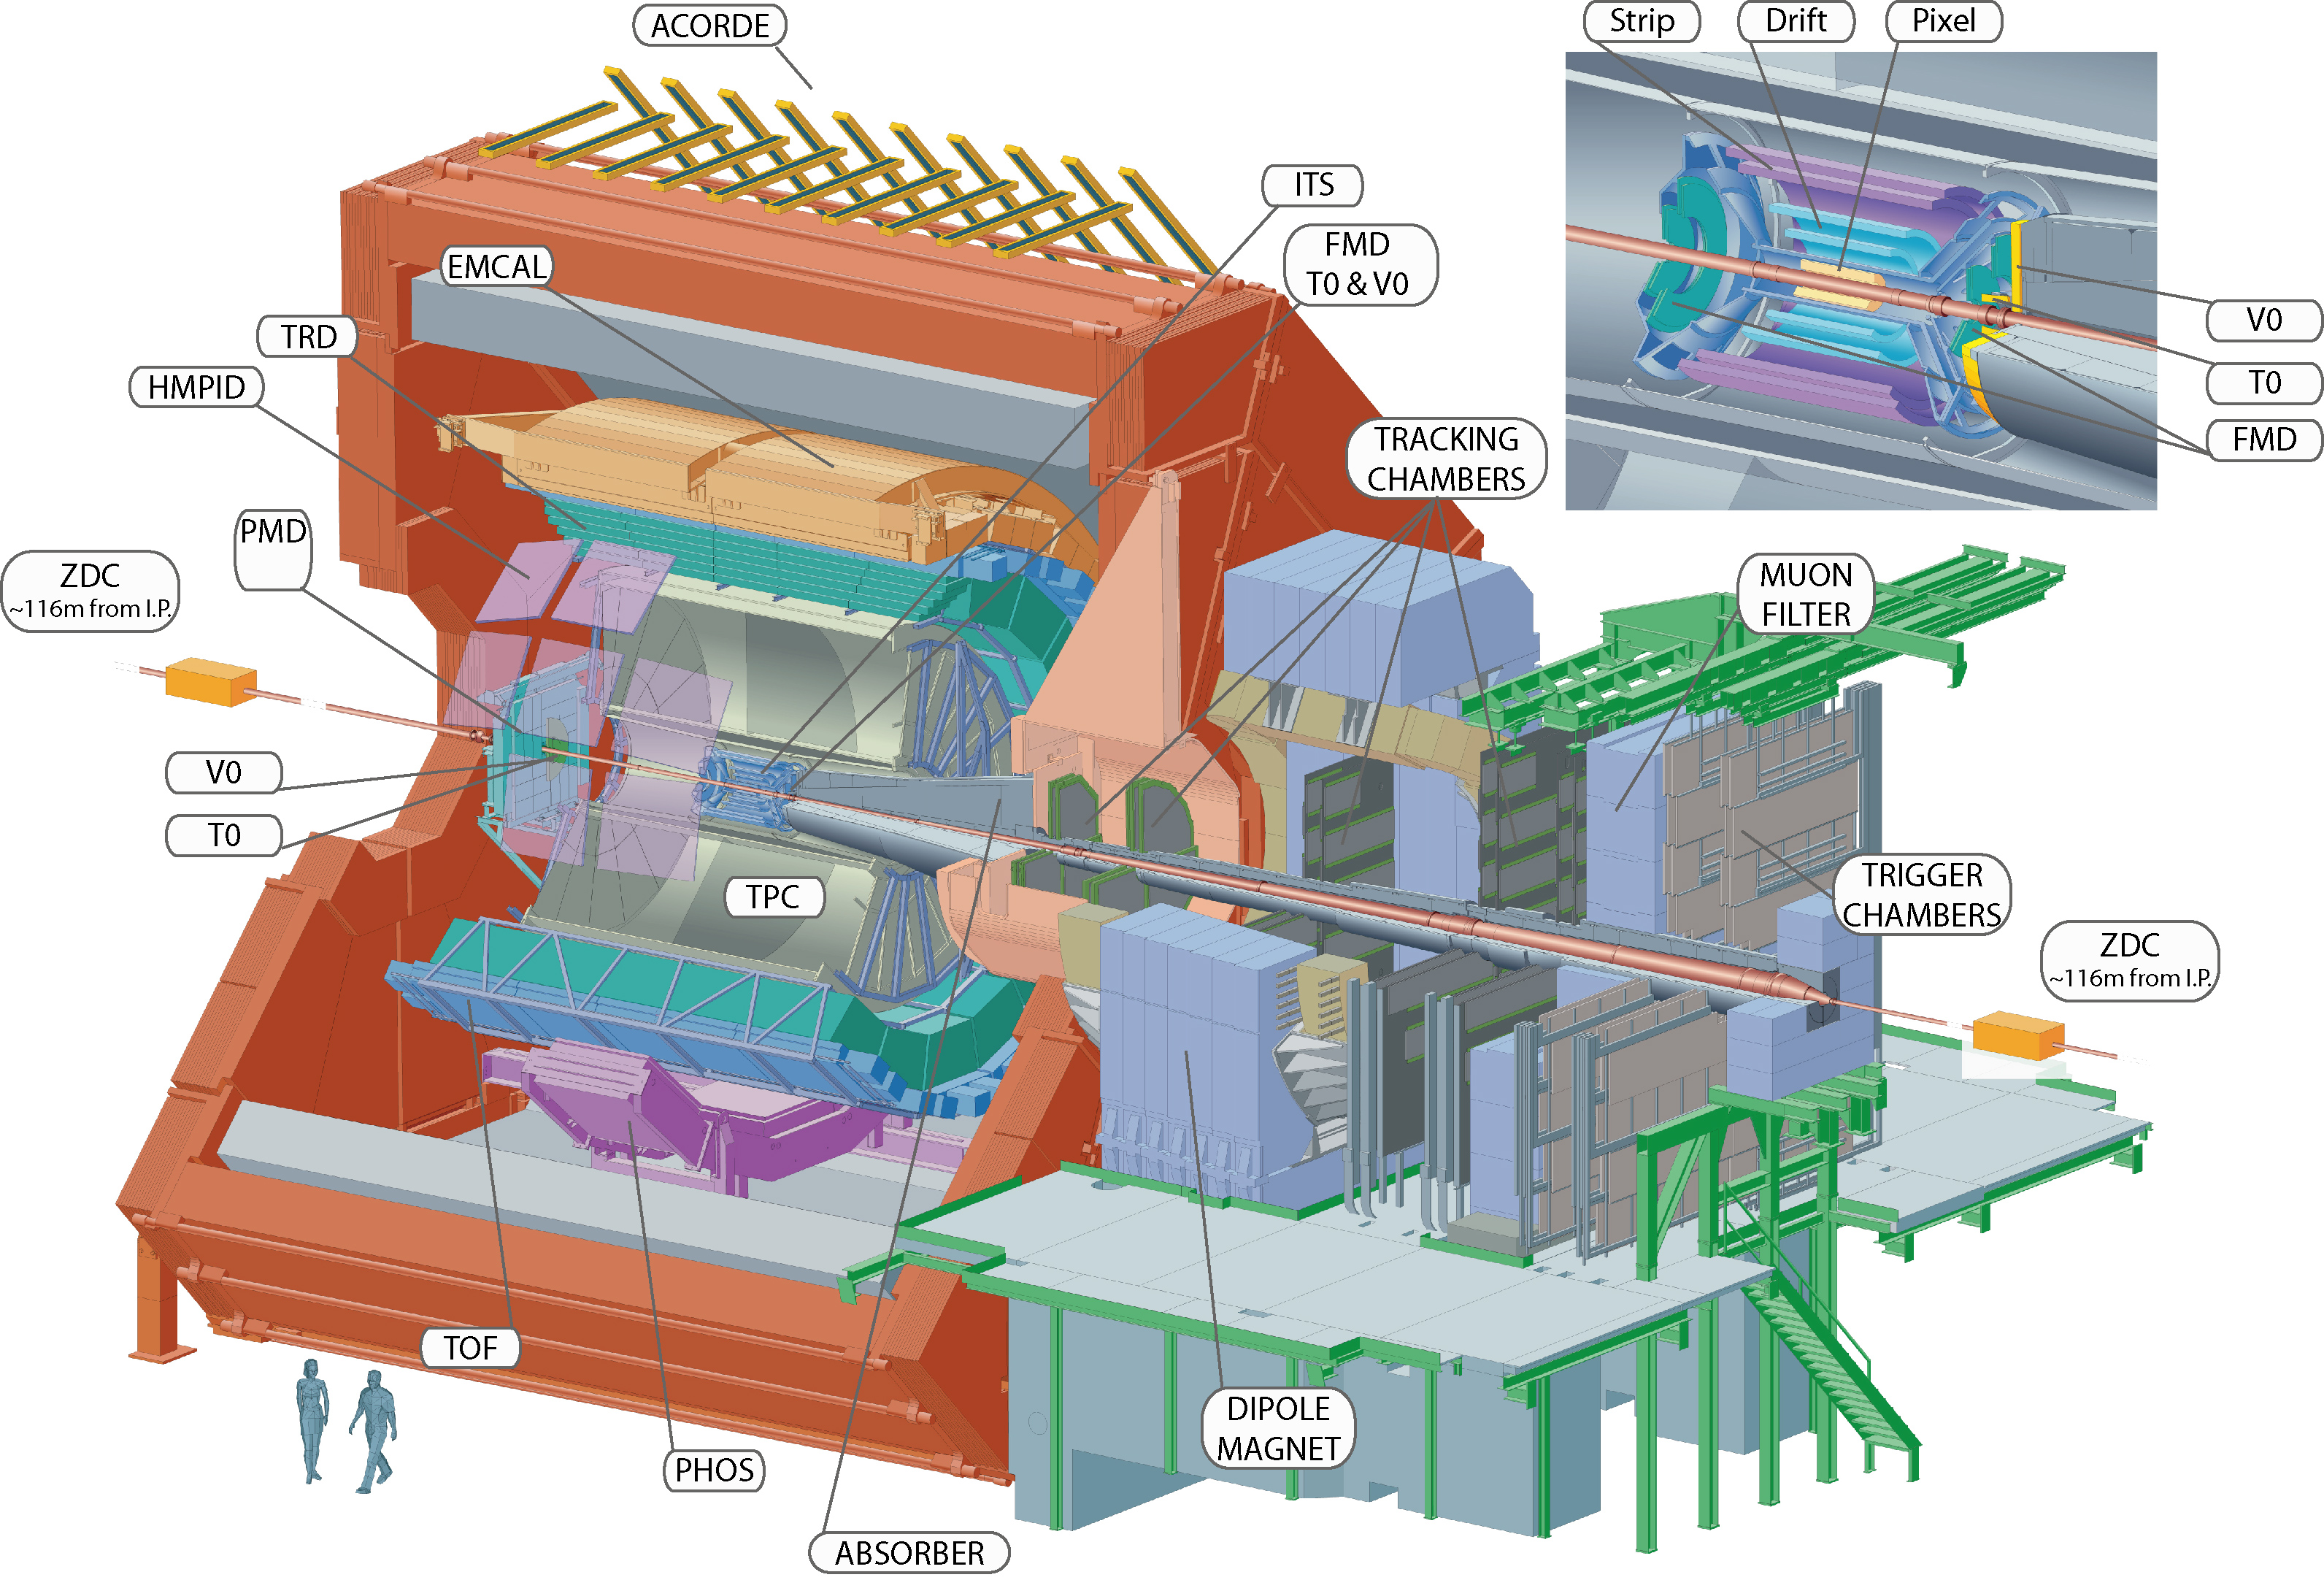
\includegraphics[width=0.85\textwidth]{gfx/alice3D}
	\caption{The ALICE experimental setup and the red L3 solenoid magnet. The top right inset shows a zoom on the V0, T0, FMD and the ITS detectors.}
	\label{fig:alice3D}
\end{figure}
The ALICE coordinate system is a right-handed orthogonal Cartesian system with the origin settled at
the nominal beams interaction point.
The $x$ axis is aligned with the horizontal accelerator plane and points to the centre of the LHC,
the $y$ axis is perpendicular to the accelerator plane and points upward.
As a consequence the $z$ axis is parallel to the beam direction and its positive direction is 
defined by the chirality of the coordinate system. 
For a more useful description of the apparatus and the physical quantities, two other coordinates
are defined, which toghether with the $z$ axis described above, form a cylindrical coordinate system:
the azimuthal angle $\phi$ increases counter-clockwise starting from $\phi = 0$ for $x$ axis looking
towards the CMS side, and the polar angle $\theta$ increases from $z$ ($\theta=0$) to $-z$ 
($\theta=\pi$).
Another usefull variable, widely used in this thesis, is the \textit{pseudo-rapidity} $\eta$:
\begin{equation}
    \eta = \frac{1}{2} \ln \frac{|p| + p_{z}}{|p| - p_{z}} =
     - \ln \left[ \tan \left(\frac{\theta}{2} \right) \right].
\end{equation}
which, for ultra-relativistic objects, numerically converges to the \textit{rapidity} already defined
in the first chapter (Section \ref{sec:1.3.2}).

\begingroup
\setlength{\tabcolsep}{6pt} % Default value: 6pt
\renewcommand{\arraystretch}{1.2} % Default value: 1
\begin{table}[!tp]\small
\centering
	\begin{tabular*}{\textwidth}{@{\extracolsep{\fill}}lcccc}
	\toprule
		     & \multicolumn{2}{c}{\normalsize{\textbf{Acceptance}}} \\
	\textbf{\normalsize{Detector}} & \textit{\textbf{Polar}} & \textit{\textbf{Azimuthal}} & \textbf{\normalsize{Position}} & \textbf{\normalsize{Main purpose}}	 \\
    \midrule
	SPD$^{\dagger}$	\textit{layer 1}     & $|\eta|$ < 2.0	  & full			& r = 3.9 cm		& tracking, vertex\\
	SPD$^{\dagger}$	\textit{layer 2}     & $|\eta|$ < 1.4	  & full			& r = 7.6 cm		& tracking, vertex\\
	SDD	\textit{ layer 3}		         & $|\eta|$ < 0.9	  & full			& r = 15 cm		    & tracking, PID\\
	SDD	\textit{ layer 4}		         & $|\eta|$ < 0.9	  & full			& r = 23.9 cm	    & tracking, PID\\
    SSD	\textit{ layer 5}			     & $|\eta|$ < 1.0	  & full			& r = 38 cm		    & tracking, PID\\
    SSD	\textit{ layer 6}			     & $|\eta|$ < 1.0	  & full			& r = 43 cm		    & tracking, PID\\
    TPC	                                 & $|\eta|$ < 0.9     & full			& 85 < r/cm < 247   & tracking, PID \\
    TRD$^{\dagger}$	                     & $|\eta|$ < 0.8     & full			& 290 < r/cm < 368  & tracking, e$^{\pm}$ id \\
    TOF$^{\dagger}$	                     & $|\eta|$ < 0.9     & full			& 370 < r/cm < 399  & PID \\
    PHOS$^{\dagger}$                     & $|\eta|$ < 0.1    & 220$^{\circ}$<$\phi$<320$^{\circ}$	& 460 < r/cm < 478 & photons \\
    EMCal$^{\dagger}$                    & $|\eta|$ < 0.7     & 80$^{\circ}$<$\phi$<187$^{\circ}$	& 460 < r/cm < 478 & photons, jets \\
    HMPID                                & $|\eta|$ < 0.6     & 1$^{\circ}$<$\phi$<59$^{\circ}$		& r = 490 cm       & PID \\
    ACORDE$^{\dagger}$                   & $|\eta|$ < 1.3     & 30$^{\circ}$<$\phi$<150$^{\circ}$   & r = 850 cm       & cosmics \\
    \midrule
    PMD		                 & 2.3 < $\eta$ < 3.9   & full			& z = 367 cm		& photons\\
    FMD 	                 & 3.6 < $\eta$ < 5.0   & full			& z = 320 cm		& ch. particles\\
			                 & 1.7 < $\eta$ < 3.7	& full			& z = 80 cm		    & ch. particles\\
			                 & -3.4 < $\eta$ < -1.7 & full			& z = -70 cm		& ch. particles\\
	V0 A$^{\dagger}$         & 2.8 < $\eta$ < 5.1	& full			& z = 329 cm		& ch. particles\\
	V0 C$^{\dagger}$         & -3.7 < $\eta$ < -1.7	& full			& z = -88 cm		& ch. particles\\
	T0 A$^{\dagger}$         & 4.6 < $\eta$ < 4.9	& full			& z = 370 cm		& time, vertex\\
	T0 C$^{\dagger}$         & -3.3 < $\eta$ < -3.0	& full			& z = -70 cm		& time, vertex\\
	ZDC$^{\dagger}$		     & $|\eta|$ > 8.8	    & full			& z = $\pm$113 cm	& fwd neutrons\\
			                 & 6.5 < $\eta$ < 7.5	& $|\phi|$<10$^{\circ}$             & z = $\pm$113 cm	&fwd protons\\
			                 & 4.8 < $\eta$ < 5.7	& $|2\phi|$<32$^{\circ}$            & z = $\pm$113 cm   &photons\\
    \midrule
	MCH	                     & -4.0 < $\eta$ < -2.5 & full & -14.2 < z/m < -5.4  & muon tracking \\
	MTR$^{\dagger}$	         & -4.0 < $\eta$ < -2.5 & full & -17.1 < z/m < -16.1 & muon trigger \\	
	\bottomrule
    \end{tabular*}
	\caption{Geometrical details and main purposes of the ALICE sub-detectors. This table has been taken and adapted from the description of the ALICE apparatus in \cite{alice:Perf2014}. The transverse (r) and longitudinal ($z$) coordinates as well as the acceptance (\textit{polar} and \textit{azimuthal}) are measured with respect to the ALICE coordinate reference frame, described in the text. When more than one position value is specified the detector is divided in two or several parts and the reported values are the minimum and maximum distances from the interaction point. The detectors marked with a dagger ($\dagger$) are also used for triggering.}
	\label{tab:alice}
\end{table}
\endgroup

In the ALICE apparatus, three main parts can be distinguished: the \textit{central barrel}, the
\textit{muon spectrometer} and the \textit{forward detectors}.

\paragraph{Central Barrel}
Consists of all the detectors located in the pseudo-rapidity range $|\eta|$ < 0.9. The central barrel 
tracking detectors include the Inner Track- ing System (ITS), the Time Projection Chamber (TPC) and the
Transition Radiation Detector (TRD), covering the full azimuthal acceptance. 
The central systems are dipped in a solenoidal magnetic field (B = 0.5 T) produced by the warm resistive
magnet previously used for the L3 experiment at LEP \cite{lep}.


